\chapter{Auswerten}
In diesem Kapitel wird die PA kritisch ausgewertet. Dabei wird auf die Erfüllung der Anforderungen eingegangen
und die Probleme, welche während der PA aufgetreten sind, beschrieben.

\section{Erfüllungsgrad der Anforderungen}
Das erhaltene Produkt dieser PA hat zwei Teile: Die Dokumentation und das Programm.
\subsection{Dokumentation}
Die Dokumentation stammt von einem Template \cite{Buhler_ipa-template_2022} ab, welches in LaTeX geschrieben
wurde: Eine ganze \enquote{Programmiersprache}, welche sich sehr gut für Dokumentationen eignet. Dinge wie der
Glossar oder das Abbildungsverzeichnis werden von LaTeX automatisch generiert. \newline
Dazu wurde auch sehr viel Wert auf das Einhalten des Kriterienkatalogs gelegt, weshalb die Dokumentation auch
sehr vollständig sein.
\subsection{Programm}
Das Programm ist ein, komplett von Redmine abgekoppeltes, Plugin. Es wurde mit ERB und Ruby geschrieben, während
die (mit 100\% coverage) Tests mit MiniTest geschrieben wurden. Auch hier werden alle Kriterien erfüllt, da die
Anforderungen als \enquote{Leitfaden} genutzt wurden. Mit einer guten Planung für die Umsetzung ging auch die
Umsetzung sehr schnell. \newline
Was nicht gelungen ist, ist das aktive Polling zu vermeiden. Das heisst, dass das Plugin nach einer SemaphoreCI
Request zu GitHub geht und diesen Dienst nach einer Commit History fragt. Dies wird unter Kapitel
\ref{sec:why_active_polling} genauer beschrieben.

\section{Reflexion}
\subsection{Probleme}
Da diese PA ein Redmine Plugin schreiben musste, wurde folgendes Problem sehr offensichtlich: Die Arbeit ist
sehr Nische, was bedeutet, dass die Dokumentation mehr oder weniger die einzige Quelle ist
\cite{redmine_plugin_tutorial}. Falls Probleme auftreten, welche von der offiziellen Dokumentation nicht
abgedeckt sind, muss man wahrscheinlich einfach selber herumprobieren. Das war auch der Fall beim SimpleCov
Setup. Für den spezifischen Fall (mit dem Redmine Framework rundherum) gibt es keine Dokumentation, GitHub
Issues oder andere Quellen im Internet. \newline
Das führte dazu, dass für das Programm sehr viel Zeit eingeplant wurde, welche am Schluss doch nicht nötig war.
\subsection{Erfolge}
Der Vorteil des oben genannten Problems war, dass die mangelnde Dokumentation das Implementieren nur noch
spannender machte. Anstatt wie für alles bisher eine Dokumentation und hundert Frameworks zu nutzen, welche einem
die ganze Arbeit abnehmen, musste selbst viel erforscht werden. Wenn etwas ging, gab es immer sehr erfüllende
Siegesmomente. \newline
Ausserhalb des Programms wurde diese IPA mit LaTeX geschrieben. Das war eine sehr gute Wahl, da sich diese
Arbeit gut dafür eignete passiv noch einen Grundkurs in LaTeX zu absolvieren.

\section{Persönliche Bilanz}
Ich fand diese PA eine meiner spannendsten Arbeiten bisher. Das lag vor allem daran, dass die Dokumentation sehr
technisch und ausführlich war. Mir wurde aber im Verlauf der Arbeit klar, dass eine agile Projektplanung für
Software besser ist. Während dem Arbeiten merkte ich oft, dass es etwas zu tun gab, was nicht im Zeitplan oder
als Arbeitspaket aufgelistet war. Das führte zu einem ungenauen Zeitplan und vielen Einträgen unter
\enquote{Puffer}.

\section{Mögliche Verbesserungen/Erweiterungen}
Das Programm wurde unter einem sehr engen Zeitplan entwickelt. Das führte dazu, dass das Programm an bestimmten
Orten gut erweiterbar ist. Einige dieser Ideen werden hier aufgelistet:
\subsection{Eigene Konventionen}
Die erste Idee war, dass der Nutzer die Konventionen selbst entscheiden kann. Es gibt in Redmine Plugins die
Möglichkeit, dass der Nutzer das Plugin einstellen kann. Das könnte man mit dem Regex für das Finden von Issue
IDs machen.
\subsection{Mehrere CI Dienste}
Das Programm könnte auch so ausgebaut werden, dass es mehrere CI Dienste unterstützt. Das wäre wichtig bei
grossen Diensten, wie zum Beispiel TravisCI.
\subsection{Richtige Zeitzonen}
Momentan zeigt das Plugin die Deployment Timestamps in UTC Zeit an. Das kann auf die Zeitzone des Nutzers
angepasst werden.
\subsection{Die Umseztung}
Damit diese Features auch wirklich umgesetzt werden, wurden auf dem GitHub Repository Issues erstellt. Diese
Issues sind mit dem Label \enquote{enhancement} markiert. Das heisst, dass es sich um eine Erweiterung handelt.
\begin{figure}
    \centering
    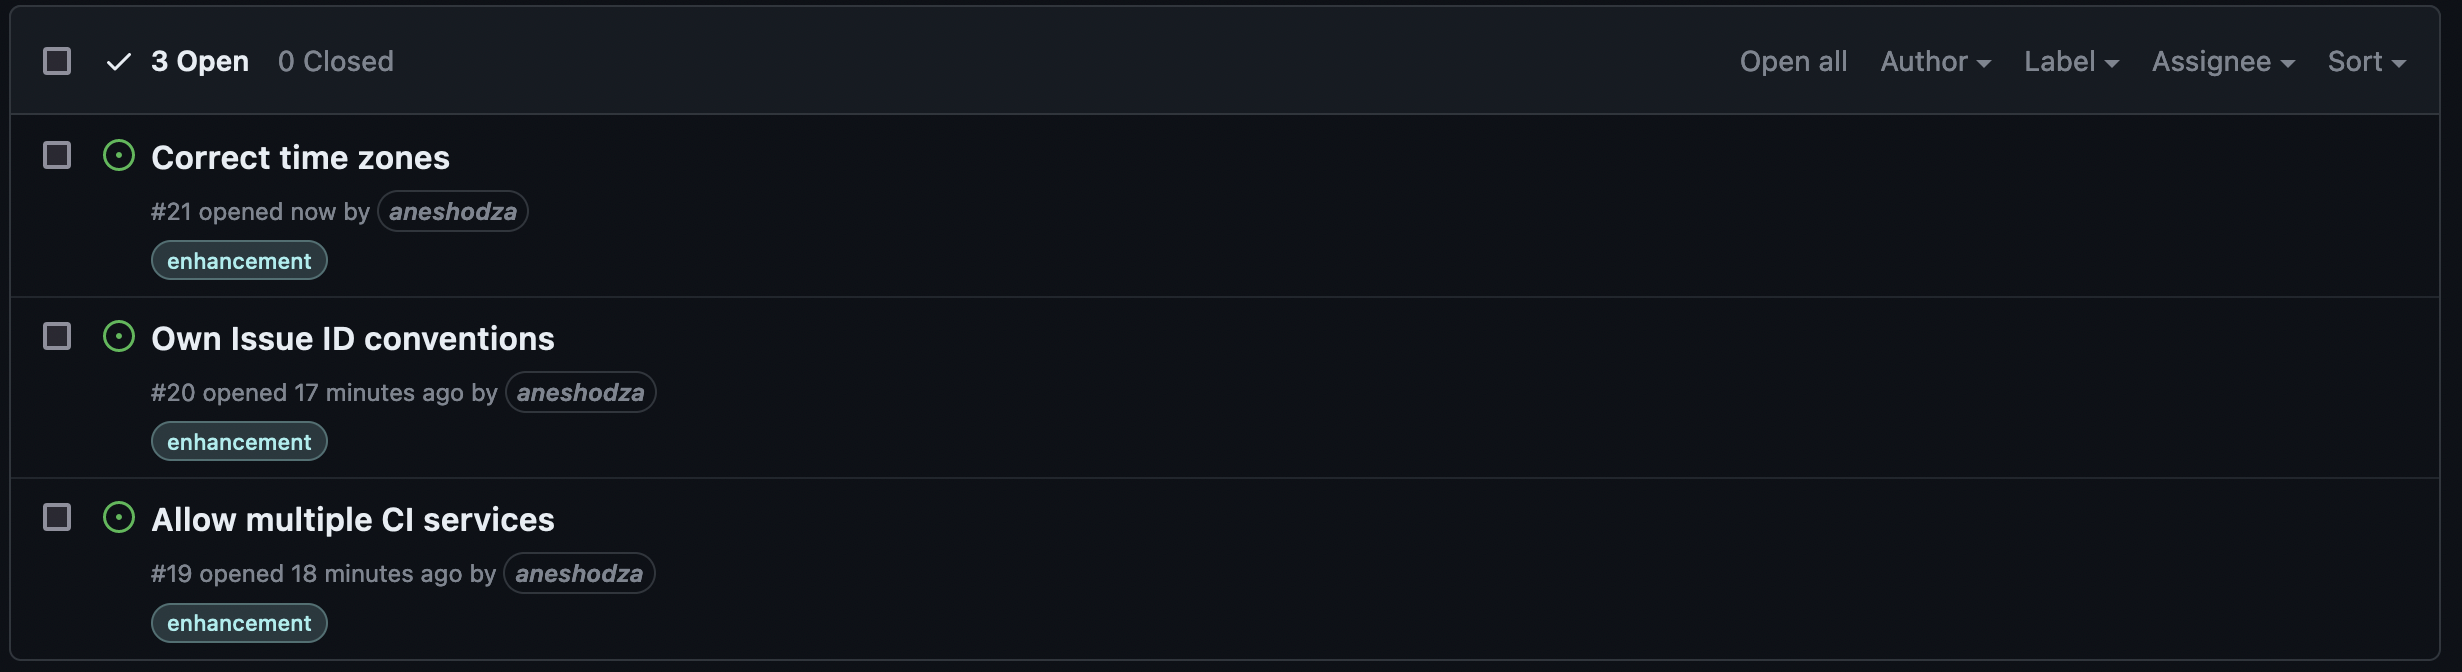
\includegraphics[width=0.75\textwidth]{images/misc/issues.png}
    \caption[Ein Screenshot von den aufgelisteten GitHub Issues]{Liste der GitHub Issues}
    \label{fig:issues}
\end{figure}
